\documentclass[../main.tex]{subfiles}
\graphicspath{{\subfix{../figures/}}}
%
\begin{document}
\section{单例模式(Singleton)}
单例模式确保某一个类只有一个实例,而且自行实例化并向整个系统提供这个实例。这个类称为\textbf{单例类}。

\textbf{单例模式的要点}:
\begin{itemize}
  \item 某个类只能有一个实例;
  \item 它必须自行创建这个实例;
  \item 必须自行向外提供这个实例。
\end{itemize}
%
在下面的对象图中,有一个``单例对象'',而``客户甲''、``客户乙''和``客户丙''是单例对象的三个客户对象。可以看到,所有的客户对象共享一个单例对象。而且从单例对象到自身的连接线可以看出,单例对象持有对自己的引用。
%
\begin{figure}[H]
  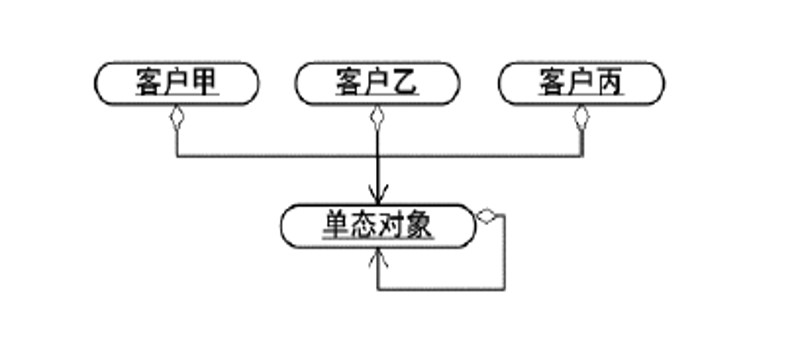
\includegraphics[width=0.50\textwidth]{18_1.jpg}
\end{figure}
%
\subsection{单例模式应用场景-资源管理}
\noindent 一些资源管理器常常设计成单例模式。
在计算机系统中,需要管理的资源包括软件外部资源,譬如每台计算机可以有若干个打印机,但只能有一个Printer Spooler,以避免两个打印作业同时输出到打印机中。每台计算机可以有若干通信端口,系统应当集中管理这些通信端口,以避免一个通信端口同时被两个请求同时调用。

\noindent 需要管理的资源包括软件内部资源,譬如,大多数的软件都有一个(甚至多个)属性(properties)文件存放系统配置。这样的系统应当由一个对象来管理一个属性文件。
需要管理的软件内部资源,比如负责记录网站来访人数的部件,记录软件系统内部事件、出错信息的部件等。这些部件都必须集中管理,不可政出多头。

\textbf{单例模式的结构}:虽然单例模式中的单例类被限定只能有一个实例,但是单例模式和单例类可以很容易被推广到任意且有限多个实例的情况,这时候称它为多例模式(Multiton Pattern)和多例类(Multiton Class)。单例类的简略类图如下所示。
\begin{figure}[H]
  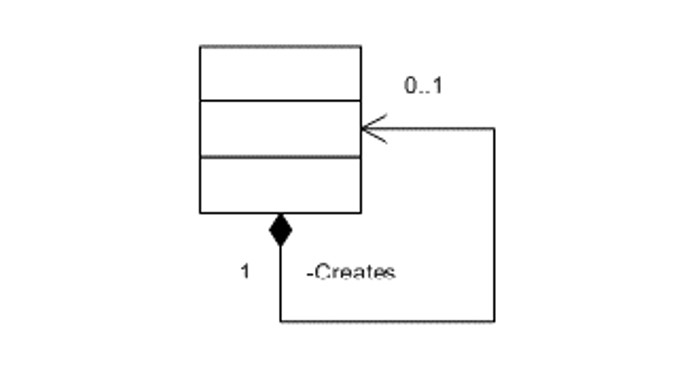
\includegraphics[width=0.55\textwidth]{18_2.jpg}
\end{figure}

\textbf{饿汉式单例类}:
\begin{lstlisting}[language=java]
public class EagerSingleton {
  private static final EagerSingleton m_instance = new EagerSingleton();
  // 私有的默认构造函数
  private EagerSingleton() {  }
  // 静态工厂方法
  public static EagerSingleton getInstance() { return m_instance; }
}
\end{lstlisting}
%
\noindent \textbf{懒汉式单例类}:与饿汉式单例类相同之处是,类的构造函数是私有的。
与饿汉式单例类不同的是,懒汉式单例类在第一次被引用时将自己实例化。
\begin{lstlisting}[language=java]
public class LazySingleton {
  private static LazySingleton  m_instance = null;
  // 私有的默认构造函数,保证外界无法直接实例化
  private LazySingleton() {  }
  // 静态工厂方法,返还此类的惟一实例
  synchronized public static LazySingleton getInstance() {
    if (m_instance == null) {
      m_instance = new LazySingleton();
    }
    return m_instance;
  }
}
\end{lstlisting}
%
\textbf{使用单例模式有一个很重要的必要条件}:
要求一个类只有一个实例时,才应当使用单例模式。
反过来说,如果一个类可以有几个实例共存,那么就没有必要使用单例类。
%
\subsection{单例类的状态}
\begin{itemize}
  \item 有状态的单例类: 一个单例类可以是有状态的(stateful),一个有状态的单例对象一般也是可变(mutable)单例对象。有状态的可变的单例对象常常当做状态库(repositary)使用。比如一个单例对象可以持有一个int 类型的属性,用来给一个系统提供一个数值惟一的序列号码,作为某个销售系统的账单号码。当然,一个单例类可以持有一个聚集,从而允许存储多个状态。
  \item 没有状态的单例类: 另一方面,单例类也可以是没有状态的(stateless),仅用做提供工具性函数的对象。既然是为了提供工具性函数,也就没有必要创建多个实例,因此使用单例模式很合适。一个没有状态的单例类也就是不变(Immutable)单例类.
\end{itemize}
%
\subsection{例子: 属性管理器}
这里给出一个读取属性(properties)文件的单例类,作为单例模式的一个实用的例子。
属性文件如同老式的windows编程时的.ini 文件,用于存放系统的配置信息。配置信息在属性文件中以属性的方式存放,一个属性就是两个字符串组成的对子,其中一个字符串是键(key),另一个字符串是这个键的值(value)。大多数的系统都有一些配置常量,这些常量如果是存储在程序内部的,那么每一次修改这些常量都需要重新编译程序。将这些常量放在配置文件中,系统通过访问这个配置文件取得配置常量,就可以通过修改配置文件而无需修改程序而达到更改系统配置的目的。系统也可以在配置文件中存储一些工作环境信息,这样在系统重启时,这些工作信息可以延续到下一个运行周期中。
假定需要读取的属性文件就在当前目录中,且文件名为singleton.properties。这个文件中有如下的一些属性项。
%
\begin{lstlisting}
// 属性文件内容
node1.item1=How
node1.item2=are
node2.item1=you
node2.item2=doing
node3.item1=?
\end{lstlisting}
%
Java 提供了一个工具类,称做属性类,可以用来完成属性文件的操作。这个属性类的继承关系可以从下面的类图中看清楚。
\begin{figure}[H]
  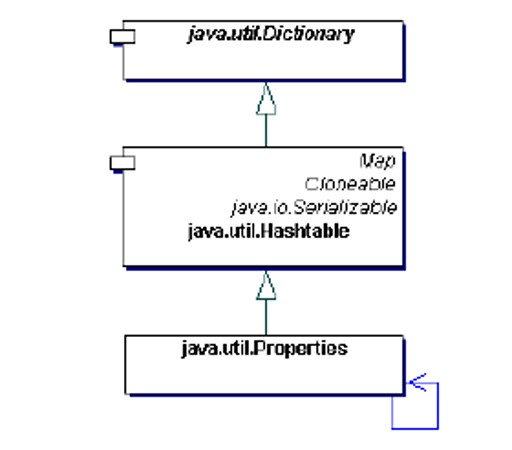
\includegraphics[width=0.55\textwidth]{18_3.jpg}
\end{figure}
%
属性类提供了读取属性和设置属性的各种方法。其中读取属性的方法有:
\begin{itemize}
  \item contains(Object value)、containsKey(Object key):如果给定的参数或属性关键字在属性表中有定义,该方法返回True,否则返回False。
  \item getProperty(String key)、getProperty(String key, String default):根据给定的属性关键字获取关键字值。
  \item list(PrintStream s)、list(PrintWriter w):在输出流中输出属性表内容。
  \item size():返回当前属性表中定义的属性关键字个数。
\end{itemize}
%
设置属性的方法有:
\begin{itemize}
  \item put(Object key, Object value):向属性表中追加属性关键字和关键字的值
  \item remove(Object key):从属性表中删除关键字。
\end{itemize}
%
从属性文件加载属性数据的方法为\texttt{load(InputStream inStream)},可以从一个输入流中读入一个属性列,如果这个流是来自一个文件的话,这个方法就从文件中读入属性。
将属性存入属性文件的方法有几个,重要的一个是\texttt{store(OutputStream out, String header)},将当前的属性列写入一个输出流,如果这个输出流是导向一个文件的,那么这个方法就将属性流存入文件。

\textbf{为什么使用单例模式}:属性是系统的一种``资源'',应当避免有多于一个的对象读写属性。此外,属性的读取可能会在很多地方发生。换言之,属性管理器应当自己创建自己的实例,并且自己向系统全程提供这一实例。因此,属性文件管理器应当是一个单例模式负责。

\textbf{系统设计}:系统的核心是一个属性管理器,也就是一个叫做ConfigManager 的类,这个类应当是一个单例类。因此,这个类应当有一个静态工厂方法,不妨叫getInstance(),用于提供自己的实例。
为简单起见,在这里采取``饿汉''方式实现ConfigManager。
%
\begin{lstlisting}[language=java]
import java.util.Properties;
import java.io.FileInputStream;
import java.io.File;
public class ConfigManager {
  // 属性文件全名
  private static final String PFILE = System.getProperty("user.dir")
  + File.Separator + "Singleton.properties";
  // 对应于属性文件的文件对象变量
  private File m_file = null;
  // 属性文件的最后修改日期
  private long m_lastModifiedTime = 0;
  // 属性文件所对应的属性对象变量
  private Properties m_props = null;
  // 本类惟一的一个实例
  private static ConfigManager m_instance =new ConfigManager();
  // 私有的构造函数, 用以保证外界无法直接实例化
  private ConfigManager() {
    m_file = new File(PFILE);
    m_lastModifiedTime = m_file.lastModified();
    if(m_lastModifiedTime == 0) {
      System.err.println(PFILE +" file does not exist!");
      System.exit(1);
    }
    m_props = new Properties();
    try {
      m_props.load(new FileInputStream(PFILE));
    } catch(Exception e) {
      e.printStackTrace();
    }
  }
  /**
  * 静态工厂方法
  * @return 返还ConfigManager 类的单一实例
  */
  synchronized public static ConfigManager getInstance() {
    return m_instance;
  }
  /**
  * 读取一特定的属性项
  *
  * @param name 属性项的项名
  * @param defaultVal 属性项的默认值
  * @return 属性项的值(如此项存在), 默认值(如此项不存在)
  */
  final public Object getConfigItem(String name, Object defaultVal) {
    long newTime = m_file.lastModified();
    // 检查属性文件是否被其他程序
    // (多数情况是程序员手动)修改过
    // 如果是,重新读取此文件
    if(newTime == 0) {
      // 属性文件不存在
      if(m_lastModifiedTime == 0) {
        System.err.println(PFILE+ " file does not exist!");
      } else {
        System.err.println(PFILE+ " file was deleted!!");
      }
      return defaultVal;
    } else if(newTime > m_lastModifiedTime) {
      // Get rid of the old properties
      m_props.clear();
      try {
        m_props.load(new FileInputStream(PFILE));
      } catch(Exception e) {
        e.printStackTrace();
      }
    }
    m_lastModifiedTime = newTime;
    Object val = m_props.getProperty(name);
    if (val == null) {
        return defaultVal;
    } else {
      return val;
    }
  }
}
\end{lstlisting}
%
下面的源代码演示了怎样调用 ConfigManager 来读取属性文件。
\begin{lstlisting}[language=java]
BufferedReader reader = new BufferedReader(
  new InputStreamReader(System.in));
System.out.println("Type quit to quit");
do {
  System.out.print("Property item to read:");
  String line = reader.readLine();
  if(line.equals("quit")) { break; }
  System.out.println(ConfigManager.getInstance()
    .getConfigItem(line, "Not found."));
} while(true);
\end{lstlisting}
%
\textbf{相关模式}:有一些模式可以使用单例模式,如抽象工厂模式可以使用单例模式,将具体工厂类设计成单例类.
\begin{lstlisting}[language=java]
DocumentBuilderFactory factory =DocumentBuilderFactory.newInstance();
DocumentBuilder builder=factory.newDocumentBuilder();
Document document=builder.parse(new File("Dom_3.xml"));
\end{lstlisting}
%
单例模式的精神可以推广到多于一个实例的情况。这时候这种类叫做多例类,这种模式叫做多例模式。单例类(左)和多例类(右)的类图如下所示。
\begin{figure}[H]
  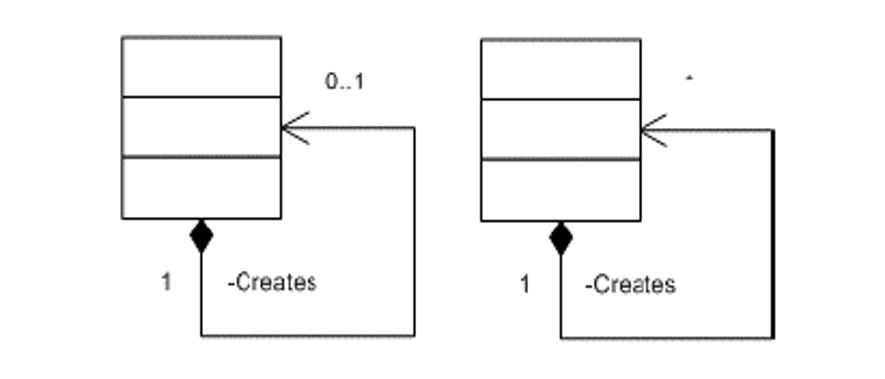
\includegraphics[width=0.50\textwidth]{18_4.jpg}
\end{figure}
%
\subsection{语言中的单例模式}
\noindent \textbf{Java 的Runtime 对象}:
在Java内部,java.lang.Runtime 对象就是一个使用单例模式的例子。

\noindent 在每一个Java应用程序里面,都有惟一的一个Runtime 对象。通过这个Runtime 对象,应用程序可以与其运行环境发生相互作用。Runtime 类提供一个静态工厂方法getRuntime()::
\texttt{public static Runtime getRuntime();}
通过调用此方法,可以获得Runtime 类惟一的一个实例:
\texttt{Runtime rt = Runtime.getRuntime();}

\noindent \textbf{Runtime 对象通常的用途包括}:
执行外部命令;返回现有内存即全部内存;运行垃圾收集器;加载动态库等。

\noindent 下面的例子演示了怎样使用Runtime 对象运行一个外部程序。
\begin{lstlisting}[language=java]
import java.io.*;
public class CmdTest {
  public static void main(String[] args)
    throws IOException {
    Process proc =  Runtime.getRuntime().exec("notepad.exe");
  }
}
\end{lstlisting}
\end{document}
